\documentclass[12pt]{article}
\title{Artomat Simulation}
\author{Nils Egger}
\date{13.08.2019}

\usepackage{listings}
\usepackage{color}
\usepackage{graphicx} 
\definecolor{dkgreen}{rgb}{0,0.6,0}
\definecolor{gray}{rgb}{0.5,0.5,0.5}
\definecolor{mauve}{rgb}{0.58,0,0.82}

\lstset{frame=tb,
  language=Python,
  aboveskip=3mm,
  belowskip=3mm,
  showstringspaces=false,
  columns=flexible,
  basicstyle={\small\ttfamily},
  numbers=none,
  numberstyle=\tiny\color{gray},
  keywordstyle=\color{blue},
  commentstyle=\color{dkgreen},
  stringstyle=\color{mauve},
  breaklines=true,
  breakatwhitespace=true,
  tabsize=3
}

\begin{document}

\maketitle
\tableofcontents 

\section{Grundidee}

Als wir auf die Idee kamen einen Roboter zu bauen und dazu eine Steuerungssoftware zu schreiben stellte ich mir die Frage wie wir dies am besten Parallel machen. Meiner Meinung nach kann man Software besser entwickeln wenn man sie auch gleich ausprobieren kann. In unserem Fall wäre dies die Kamera auf den aufgehängten Roboter mit den Erkennungspunkten zu richten. Mit diesen Gedanken im Kopf kam ich auf die Idee eine Simulation zu schreiben während David an unserem Roboter arbeitet.

\section{Installation}
\subsection{Voraussetzungen}
\begin{enumerate}
\item Python Version $\geq 3.6$\newline
https://www.python.org/downloads/
\item Python Bibliotheken \newline
Nach dem Download von Python müssen wir noch folgende Bibliotheken installieren. 
\begin{itemize}
	\item tkinter
	\item numpy
	\item Pillow
\end{itemize}
Der Konsolen Command funktioniert folgenderweise:
\begin{lstlisting}
pip install <bibliothek>
\end{lstlisting}
\end{enumerate}
Falls Sie den IDPA Ordner mit all Code noch nicht vor sich haben und git auf Ihrem Computer installiert haben, dann können Sie ganz einfach mein Repository clonen:
\begin{lstlisting}
git clone https://github.com/nilsegger/idpa.git
\end{lstlisting}
\subsection{Skript Starten}
Starten Sie wieder eine Konsole und wechseln Sie den Pfad zum Skript Ordner. Stellen Sie sicher, dass Sie das Skript "simulation.py" im Ordner sehen. Starten Sie dann dieses mit:
\begin{lstlisting}
python simulation.py
\end{lstlisting}
Falls Sie eine Fehlermeldung von fehlenden Paketen (Bibliotheken) überkommen, installieren Sie diese bitte auch noch. Falls Sie danach trotzdem noch eine Fehlermeldung überkommen, schreiben Sie mir doch bitte eine Email \newline nils.egger@stud.bbbaden.ch.
\subsection{Visuelle Erklärung}
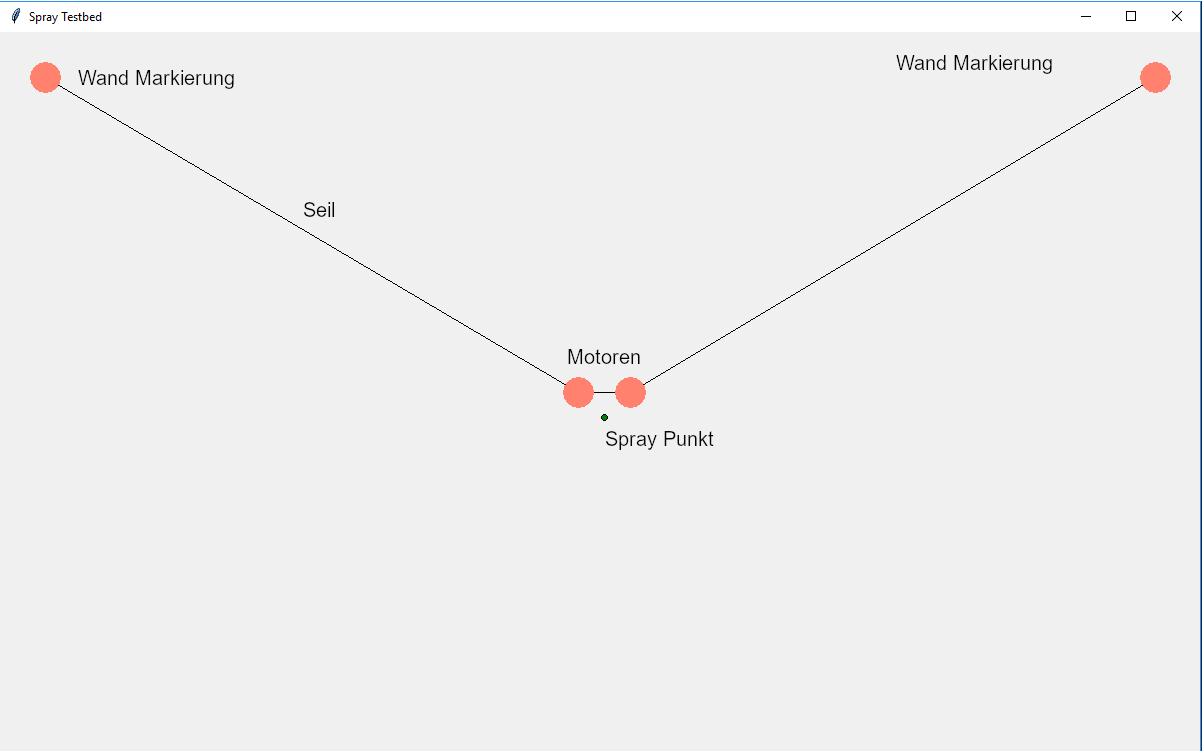
\includegraphics[width=1\textwidth]{simulation_visuelle_erklaerung.PNG}
Die Roten Punkte imitieren die LEDs welche an der Wand und am Roboter befestigt sind. Diese müssend dann von unserem Navigationsskript korrekt erkannt werden damit ein Bild überhaupt gesprayed werden kann.
\subsection{Steuerungen}
Die Simulation lässt sich über folgende Tastaturdrücke steuern.
\begin{itemize}
	\item \textbf{W} \newline
	Mit W dreht sich der linke Motor auf, somit wird das linke Seil kleiner.
	\item \textbf{S} \newline
	Mit S gibt der linke Motor nach, somit wird das linke Seil grösser.
	\item \textbf{$\uparrow$} \newline
	Mit $\uparrow$ dreht sich der rechte Motor auf, somit wird das rechte Seil kleiner.
	\item \textbf{$\downarrow$} \newline
	Mit $\downarrow$ gibt der rechte Motor nach, somit wird das rechte Seil grösser.
	\item \textbf{Q} \newline
	Mit Q wird die Wand (in diesem Fall Canvas) mit einem Punkt bemalt.
\end{itemize}

\section{Bibliotheken}
Für die Simulation gebrauche ich Tkinter für die Darstellung. Im Nachhinein war dies vermutlich ein fehlentschluss, dies nicht weil die Bibliothek die Simulation schlecht darstellt, sondern weil sie die Darstellung nicht einfach in eine Pixel Matrix kopieren kann.
Müsste ich nochmals eine auswahl treffen, so würde diese bei OpenCV liegen, denn mit OpenCV hätte ich nur kleine Performance Verluste beim Transport des Bildes zum Navigationsalgorithmus gehabt. Dies wusste ich im voraus nicht da ich weder mit OpenCV oder Tkinter bekannt war, in Zukunft wird dies aber ein No-Brainer.
Damit ich eine Kamera auf die Simulation simulieren konnte, musste ich den Tkinter Canvas in das einzig Unterstüzte Format exportieren, nähmlich Postscript ein Vektor Format. Postscript wird jedoch natürlich nicht von OpenCV unterstützt und anstatt eine Kamera einfach auf den Bildschirm zu richten, musste ich eine weitere Bibliothek benutzen. PIL (Python Imaging Library) kam hierbei zur Lösung, diese Bibliothek kann Postscript in ein normales Bild verwandeln welches von Numpy (Matrix Bibliothek, welche von OpenCV für die Pixel Matrix von Bildern benutzt wird.) dann als Multidimensionaler Array eingelesen wird und von OpenCV bereit ist.
Dies entspricht folgendem Code:
\begin{lstlisting}
numpy.array(Image.open(io.BytesIO(self.ps_frame.encode('utf-8'))))
\end{lstlisting}
Diese eine Linie Code entnimmt dem Navigationsskript jegliche Möglichkeit bei 60 Bildern pro Sekunde zu arbeiten.

\section{Aufbau}
Die Simulation besteht aus folgenden Klassen:
\begin{enumerate} 
\item \textbf{Window}\newline
Die Window Klasse ist unter anderem dafür zuständig einen Canvas für die Simulation bereit zu stellen und diesen gleichzeitig per Interface Funktion an OpenCV weiterzugeben.
Die Hauptfunktion ist jedoch die Endlos Schleife zu steuern, diese wird von Tkinter durch folgende Funktion übernommen:
\begin{lstlisting}
Tk().after(zeit_in_ms, callback_funktion)
\end{lstlisting}
Bei jeder Wiederholung wird die vergangene Zeit gemessen und anhand von abgefangen Tastenschlägen die Geschwindigkeit der Motoren in der Simulation festgelegt.
\item \textbf{Simulation}\newline
Die Simulation Klasse ist das Herzstück dieses Skripts. Sie berechnet die Positionen des Robotors und zeichnet dieser auch gleich auf dem bereitgestellten Canvas von der Window Klasse.
\item \textbf{Object}\newline
Ursprünglich hatte ich die Idee ganz viele kleinere Klassen zu schreiben. Im Sinne das der Motor eine eigene Klasse wäre und der Spraykopf auch. Diese Objekte würden dann alle vom Window gezeichnet werden. Dieser Anlauf hatte ich dann aber auch schnell wieder geändert, nun ist es so, dass die Simulation Klasse eine Kinderklasse der Object Klasse ist und somit alle Funktionen erbt. Die Object Klasse hat Funktionen wie zum Beispiel die Distanz zwischen zwei Vektoren zu kalkulieren oder eine Linie auf einen Canvas zu zeichnen.
\item \textbf{Vec2}\newline
Die Vec2 Klasse beinhaltet Hilfsfunktionen für Rechnungen mit einem 2 Dimensionalen Vektor, diese Funktionen sind unter anderem die Länge des Vektor zu berechnen, den Vektor zu drehen oder zwei Vektoren zusammen zu rechnen.
\item \textbf{ObjectDimension}\newline
Der Name dieser Klasse beschreibt vielleicht nicht so gut was sie genau macht. Diese Klasse speichert nur zwei Vektoren, die Position und Grösse eines Objekts der Simulation (zum Beispiel der Motoren), zudem hat es eine Hilfsfunktion um die Mitte eines Objekts dieser Klasse zu berechnen.
\end{enumerate}
\section{Simulation Physik}

Bei der Physik der Simulation war für mich Wichtig, dass diese so echt wie möglich ist. Dies ist mir meiner Meinung nach im zweiten Versuch gut gelungen. Ich wollte das sich die Seile anfühlen wie Seile, damit meine ich zum Beispiel, dass wen man mit dem Linken Motor das linke Seil anzieht, dass dieses auch ein bisschen oberhalb des rechten ist, weil die Gravitation das rechte Seil mit dem Gewicht des Roboters noch runter zieht.
\subsection{Demonstration}
\textbf{Startposition:}\newline
\includegraphics[width=1\textwidth]{demonstration/simulation_start.PNG}
\textbf{Linker Motor angezogen:} \newline
\includegraphics[width=1\textwidth]{demonstration/linker_motor_angezogen.PNG}
Wie Sie sehen ist die Linie welche ich mit Gelb angestrichen habe nicht mehr gerade. Dies sieht vielleicht nicht nach viel aus, war aber für mich ein grosser Erfolg. Der linke Motor wurde angezogen, jedoch nur so viel, dass der rechte Motor noch am gleichen Ort bleibt, weil die Verbindung zwischen den zwei Motoren immer noch gleich lang ist, wäre der linke Motor noch weiter hoch gezogen worden, so wäre auch der rechte Motor verschoben.\newline \newline
\textbf{Extremfall:} \newline
Der rechte Motor dreht sich aus und der Linke Motor dreht sich ein. Das rechte Seil ist lang und das linke ist kurz.\newline
\includegraphics[width=1\textwidth]{demonstration/extremfall1.PNG}
\includegraphics[width=1\textwidth]{demonstration/extremfall2.PNG}
\textbf{Umgekehrt noch:}\newline
\includegraphics[width=1\textwidth]{demonstration/extremfall3.PNG}

Wie Sie vermutlich schon selbst bemerkt haben funktioniert die Simulation nicht mehr flüssig in diesen Extremfällen, darüber werde ich weiter unten noch mehr erzählen.

\subsection{Code Erklärung}
Die Simulation wird über zwei wichtige Funktionen gesteuert,
\begin{lstlisting}
def spin_left_motor(self, speed):
	pass
def spin_right_motor(self, speed):
	pass
\end{lstlisting}
Diese zwei Funktionen sind verkehrte Kopien von Einander, darum werde ich nur eine von beiden erklären, nämlich die Linke Seite.
Wichtig zu wissen vielleicht, diese Funktionen werden in der Hauptschleife von Window immer wieder aufgerufen bei den richtigen Tastenschläfen. Somit basiert sie darauf, dass sie immer wieder nacheinander aufgerufen wird. \pagebreak

\begin{lstlisting}
def spin_left_motor(self, speed):

	""" 
	Bei negativer Geschwindigkeit verkleinert sich das Seil, somit wird bei positiver Geschwindigkeit das Seil natuerlich groesser.
	
	
	has_rope_tension() testet ob die Laengen der zwei Seile plus der Anfangsabstand der zwei Motoren gleichgross oder kleiner als der Abstand zwischen den zwei Wand Markierungen ist. Wenn Wahr, kann man die Motoren nicht weiter anspannen weil sonst das Seil reissen wuerde. Somit wird die Funktion fruehzeitig verlassen.
	"""
	if speed < 0 and self.has_rope_tension():
		return
	
	"""
	Position und zwischengespeicherte Seil Laenge werden auf gewuenschte Position/ Laenge veraendert.
	"""
	self.left_rope_distance += speed
	self.motor_left.pos.add(self.motor_left_to_left_corner_vec, speed)
	
	# noch unwichtig.
	self.slow_forward = 0.05
	self.medium_forward = 0.1
	self.fast_forward = 1
	self.faster_than_fast_forward = 1.25
	
	if speed < 0:
		pass
	else:
		pass
	
\end{lstlisting}
Nun wird die Funktion in zwei Richtungen aufgeteilt, wenn der Motor aufgerollt wird oder eben ausgerollt. Zuerst erkläre ich den Algorithmus für das Aufrollen des Seiles (speed $< 0$).

Beim Aufrollen des Seiles wird wieder in zwei verschiedene Situation aufgeteilt.
\begin{enumerate}
	\item Seile sind noch Locker. Roboter zieht noch die Seile runter, erkennbar dadurch, dass sich die beiden Seile noch überkreuzen könnten.
	\item Seile werden langsam richtig gespannt, diese Situation wird erreicht wenn sich die beiden Seile nicht mehr überkreuzen könnten.
\end{enumerate}

\begin{lstlisting}
...
if speed < 0:
	if self.ropes_intercept:
		# Situation Seile koennen sich noch ueberkreuzen. (1)
		pass
	else:
		# Situation Seile koennten sich nicht mehr ueberkreuzen. (2)
		pass
\end{lstlisting}

Stellen Sie sich nun vor der linke Motor wird angespannt und die Seile sind immer noch locker, somit sind wir in der ersten Situation.
Nun ist die Frage ob der rechte Motor vom linken Motor mitgezogen wird oder nicht. Um dies herauszufinden misst man den neuen Abstand zwischen den zwei Motoren und vergleicht ihn mit dem Startabstand dieser zwei. Ist der neue Abstand grösser so muss der rechte Motor nachgeschoben werden. Unser Zwischenstand:
\begin{lstlisting}
...
if speed < 0:
	if self.ropes_intercept:
		while self.current_motor_to_motor_distance > self.motor_to_motor_starting_distance:
			pass
\end{lstlisting}
Nun müssen wir nur noch den rechten Motor nachschieben. Dieser Motor darf sich jedoch nur um die rechte Wandmarkierung im Radius der Länge des rechten Seiles bewegen. Visuell mit Gelb gekennzeichnet:\newline
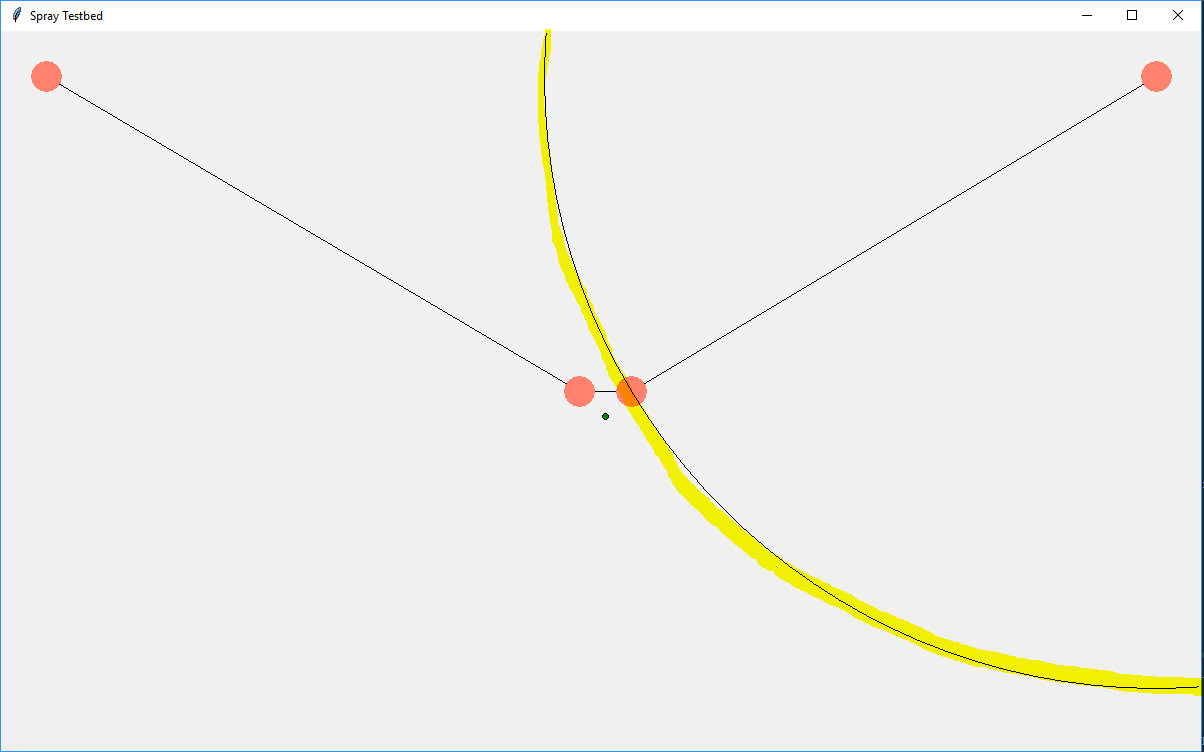
\includegraphics[width=1\textwidth]{motor_wanderlinie.PNG}
Für diese Bewegung gibt es für beide Motoren wieder eine gegenseitige kopierte Funktion. Hier ist die Erklärung für die Bewegung des linken Motores.
\begin{lstlisting}
def move_left_motor(self, degree: float, forward: float):
	distance_to_corner = self.current_left_motor_to_corner_distance
	"""
		Hier wird der Richtungsvektor von der Linkenmarkierung zum Motor berechnet, dieser wird dann um die gewuenschte Grad (degree) anzahl gedreht.
	"""
	rotation_vec = self.calculate_vec(self.corner_left.center, self.motor_left.center)
	rotation_vec.rotate(degree)
	"""
		Neuer Punkt wird erstellt und ein neuer Richtungsvektor vom Motor zu diesem Punkt wird berechnet,
		danach wird dieser neuer Richtungsvektor dem Motor hinzugefuegt. Der Motor ist jetzt am neuen gewuenschten Punkt.
	"""
	rotated_point = Vec2(copy=self.corner_left.center)
	rotated_point.add(rotation_vec, distance_to_corner)
	forward_vec = self.calculate_vec(self.motor_left.center, rotated_point)
	self.motor_left.pos.add(forward_vec, forward)
	"""
		Hier wird die Position noch korrigiert, da die neue Position einbisschen innerhalb des Kreises liegt,
		muss der neue Punkt noch einbisschen nach aussen korrigiert werden. Sonst wuerde der Motor irgendwann bei der Wandmarkierung sein.
	"""
	self.motor_left.pos.add(rotation_vec, distance_to_corner - self.current_left_motor_to_corner_distance)
\end{lstlisting}
Nun zurück zum nachschieben des rechten Motores, dies sieht nun folgenderweise aus. Dieser drehen wir nun in die richtige Richtung und schauen zudem das er nicht überschiesst, im Sinne das der rechte Motor immer tiefer oder auf der gleichen Höhe wie der linke Motor bleibt.
\begin{lstlisting}
...
if speed < 0:
	if self.ropes_intercept:
		while self.current_motor_to_motor_distance > self.motor_to_motor_starting_distance and self.motor_right.center.y >= self.motor_left.center.y:
			self.move_right_motor(1, self.slow_forward)
			# Falls der Motor hoeher als der Linke wurde, wird der Motor wieder zurueck positioniert.
			if self.motor_right.center.y < self.motor_left.center.y:
				self.move_right_motor(-1, self.slow_forward)
				break
\end{lstlisting}

Nun kann es passieren, dass der rechte Motor bis auf die gleiche Höhe wie der linke Motor nachgeschoben wurde, jedoch sind sie immer noch weiter auseinander als sie in Echt sein könnten. Dies wird wieder mit dem originalen Abstand versus dem momentan Abstand der Motoren bestimmt. Um den Abstand wieder zu korriegieren muss man den linken Motor seiner Linie nach, nach oben verschieben, bis der kleinst mögliche Abstand erreicht wird.

\begin{lstlisting}
...
if speed < 0:
	if self.ropes_intercept:
			while self.current_motor_to_motor_distance > self.motor_to_motor_starting_distance and self.motor_right.center.y >= self.motor_left.center.y:
				self.move_right_motor(1, self.slow_forward)
				# Falls der Motor hoeher als der Linke wurde, wird der Motor wieder zurueck positioniert.
				if self.motor_right.center.y < self.motor_left.center.y:
					self.move_right_motor(-1, self.slow_forward)
					break
					
		last_motor_distance = self.current_motor_to_motor_distance
		while self.current_motor_to_motor_distance > self.motor_to_motor_starting_distance and last_motor_distance >= self.current_motor_to_motor_distance:
			last_motor_distance = self.current_motor_to_motor_distance
			self.move_left_motor(-1, self.slow_forward)
		if last_motor_distance < self.current_motor_to_motor_distance:
		self.move_left_motor(1, self.slow_forward)
\end{lstlisting}
Dies ist der Fertige Code für die erste Situation. Bei der zweiten Situation, wenn die Seile gespannt sind und sich nicht mehr überkreuzen könnten, wird einfach der rechte Motor nachgeschoben bis er die gleiche Höhe wie der linke erreicht, danach ergibt sich aber schnell wieder das gleiche Problem, die Motoren sind zu weit auseinander. Als Lösung wird der linke Motor ein bisschen hochgeschoben und der rechte nachgeschoben bis er wieder die gleiche Höhe erreicht. Dies funktioniert weil die Endpunkte der Seile oben am nächsten beieinander sind.
\begin{lstlisting}
...
if speed < 0:
	if not self.ropes_intercept:
		while self.motor_right.center.y > self.motor_left.center.y:
			self.move_right_motor(1, self.slow_forward)
		while self.current_motor_to_motor_distance > self.motor_to_motor_starting_distance and not self.has_rope_tension():
		self.move_right_motor(1, self.slow_forward)
			while self.motor_right.center.y < self.motor_left.center.y:
				self.move_left_motor(-1, self.slow_forward)
\end{lstlisting}
Als letztes gibt es natürlich noch die Situation, wo die Motoren nachlassen und das Seil länger wird. Wenn der linke Motor runter gelassen wird, schaut man zuerst, ob die Motoren Distanz kleiner als der Ursprüngliche Abstand ist. Falls dies der Fall ist, so wird der linke Motor runter gelassen, bis der Abstand erreicht wird. Nun muss der rechte Motor noch nachgeschoben werden, da dieser vom linken mit runter gezogen wird.
\begin{lstlisting}
...
if speed > 0:
	while self.current_motor_to_motor_distance < self.motor_to_motor_starting_distance:
		self.move_left_motor(1, self.slow_forward)
		while self.motor_right.center.y < self.motor_left.center.y <= self.corner_right.center.y + self.right_rope_distance:
			self.move_right_motor(-1, self.fast_forward)
\end{lstlisting}
Nur mit diesem Code ergibt sich das Problem, dass es sich nicht wirklich echt anfühlt, der Motoren Abstand zu gross wird und die Simulation in der Nähe vom unteren Ecken komplett spinnt. Visuell: \newline
\includegraphics[width=1\textwidth]{fehler.PNG}
Wie man sieht wäre dies in Echt nicht so. Der linke Motor wurde gerade nach unten hängen. Um dies zu erreichen, erkenne ich den Moment, wo beide Motoren den gleichen Richtungsvektor (Länge bei beiden auf 1 berechnet) zur rechten Wandmarkierung aufweisen. Danach ist es nur noch eine Frage des Motores Abstands welcher noch korrigiert werden muss.
\begin{lstlisting}
...
if speed > 0:
	while self.current_motor_to_motor_distance < self.motor_to_motor_starting_distance:
		self.move_left_motor(1, self.slow_forward)
		while self.motor_right.center.y < self.motor_left.center.y <= self.corner_right.center.y + self.right_rope_distance:
			self.move_right_motor(-1, self.fast_forward)
			
	left_motor_to_right_corner_vec = self.calculate_vec(self.corner_right.center, self.motor_left.center)
	right_motor_to_right_corner_vec = self.calculate_vec(self.corner_right.center, self.motor_right.center)
	
	while self.current_motor_to_motor_distance > self.motor_to_motor_starting_distance \
	and not left_motor_to_right_corner_vec.compare(right_motor_to_right_corner_vec, 2):
		self.move_right_motor(1, self.faster_than_fast_forward)
	
	left_motor_to_right_corner_vec = self.calculate_vec(self.corner_right.center, self.motor_left.center)
	right_motor_to_right_corner_vec = self.calculate_vec(self.corner_right.center, self.motor_right.center)
	
	if self.current_motor_to_motor_distance > self.motor_to_motor_starting_distance:
		motor_to_motor_forward = self.calculate_vec(self.motor_right.center, self.motor_left.center)
		new_pos = Vec2(copy=self.motor_right.pos)
		new_pos.add(motor_to_motor_forward, self.motor_to_motor_starting_distance - 0.1)
		self.motor_left.pos = new_pos
		self.left_rope_distance = self.calculate_length(self.motor_left.center, self.corner_left.center)
\end{lstlisting}

\subsection{Probleme}
Der Code war während der Entwicklung extrem anfällig für Endlosschleifen, dies konnte ich aber mit der Zeit gut beheben. Die Simulation ist zudem nicht sehr genau, dies liegt darin, dass die Position nicht wirklich berechnet werden, sondern solange herum geschoben wird, bis die Position allen Anforderungen (Motoren Abstand oder zum Beispiel, dass der einte Motor nicht höher sein darf) entspricht. Der Code läuft zudem nicht immer so flüssig wegen der Bewegungsfunktion für die Motoren. Diese Funktion gebraucht nicht lange zum berechnen der neuen Position, sondern macht dies Ungenau. Durch die Ungenauigkeit werden zum Teil Positionen erreicht, welche nicht den Anforderungen entsprechen, und als Folge haben, dass der Code die Position korrigieren muss. Die neue korrigierte Position wurde aber genau gleich erreicht, nämlich mit der ungenauen Funktion, somit sind wir wieder genau gleich weit. Nun stellt man sich vielleicht die Frage, warum die Bewegungsfunktion nicht besser geschrieben wurde. Wie oben schon beschrieben wurde, funktioniert sie in dem man zuerst den Richtungsvektor zur Wandmarkierung misst, diesen um eine gewünschte Anzahl Grad dreht, in unserem Fall immer 1 Grad, diesen Richtungsvektor der Wandmarkierung hinzurechnet und danach einen neuen Richtungsvektor berechnet zwischen dem zu bewegenden Motor und dem neu berechneten Punkt. Danach wird die Länge des Richtungsvektors auf 1 berechnet und die Distanz, welche man den Motor bewegen will, dazu berechnet. Bei dieser letzten Bewegung geht die Rundung des Kreises verloren und man muss die Position, besser gesagt die Distanz zur Wandposition, korrigieren. Dies ist ungenau. Viel besser wäre es wie vorher den Richtungsvektor zwischen Motor und Wandmarkierung zu messen und diesen um weniger als 1 Grad zu drehen. Danach müsst man den Richtungsvektor ganz einfach wieder der Wandmarkierung hinzufügen und der neue Punkt wäre bereits perfekt getroffen worden. Das Problem liegt beim rotieren des Vektors, wenn der Wert des Grades kleiner als eins war, so berechnete Python die neuen Werte komplett falsch. Somit musste ich eine andere Variante finden.


\end{document}